\begin{figure}[htbp]
\centering
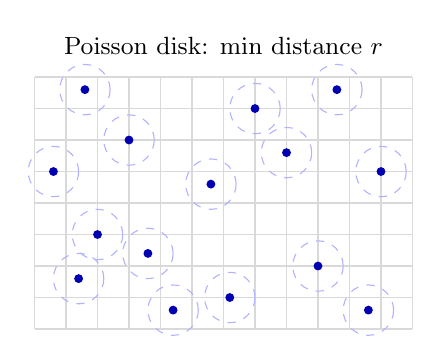
\begin{tikzpicture}[scale=0.8]
  \draw[gray!30,thin] (0,0) grid[step=0.5] (6,4);
  \foreach \x/\y in {0.7/0.8, 1.8/1.2, 3.1/0.5, 4.5/1.0, 5.3/0.3, 0.3/2.5, 1.5/3.0, 2.8/2.3, 4.0/2.8, 5.5/2.5, 1.0/1.5, 3.5/3.5, 4.8/3.8, 2.2/0.3, 0.8/3.8} {
    \fill[blue!70!black] (\x,\y) circle (2pt);
    \draw[blue!30,thin,dashed] (\x,\y) circle (0.4);
  }
  \node[font=\small] at (3,4.5) {Poisson disk: min distance $r$};
\end{tikzpicture}
\caption{Poisson disk sampling: points are placed with minimum distance $r$ between any pair.}
\label{fig:poisson_disk}
\end{figure}
